\chapter{Wissensrepräsentationsformen}
\label{chap:wissensrepFormen}

Nach Darstellung der Grundlage von Graphen und Graphdatenbanken im letzten Kapitel, wollen wir jetzt Repräsentationsformen von Wissen analysieren.\\
In der Wissensmodellierung (Knowledge-Engineering) gibt es verschiedene Formen der Wissensrepräsentation um Wissen in wissensbasierten Systemen formal abzubilden. Auf diese Art abgelegte Informationen werden als Wissensdatenbank bzw. Wissensbasis bezeichnet (vgl.~\cite{wikiWissensrep}).

Das folgende Kapitel basiert auf~\cite[S. 85 - 90]{laemmel} und beschreibt einige klassische Formen der Wissensrepräsentation, nämlich semantische Netze, Wissensnetze und Frames.

Im Gegensatz zu Regeln stehen hier die Objekte und nicht Zusammenhänge und logische Abhängigkeiten im Vordergrund.

Semantische Netze und Frames versuchen das menschliche Gedächtnis abzubilden. Sie wurden hauptsächlich zur Analyse von Wörtern und Sätzen verwendet. Ein weiterer Aspekt ist die verständliche Darstellung von Klassen und ihren Beziehungen. Die Konzepte der semantischen Netze und Frames haben die Entwicklung der objektorientierten Programmierung beeinflusst.

\section{Semantische Netze}
\label{sec:wissensrepFormen_semantischeNetze}

Eine zusammengehörige Gruppe von Objekten wird als Klasse bezeichnet. Ein einzelnes Objekt heisst Individuum. Es gibt Beziehungen zwischen Objekten, zwischen Objekten und Klassen und zwischen Klassen.

Folgende Beziehungen werden unterschieden:
\begin{itemize}
    \item ``ist ein'' Relation

        Es handelt sich um Ober- und Unterklassen.

        Beispiel: \textit{Eine Abenteuerreise ist eine Reise.}

    \item ``Instanz von'' Relation

        Die Relation sagt aus von welchem Typ ein Individuum ist.

        Beispiel: \textit{Seilpark Balmberg ist eine Instanz der Klasse Ausflug.}

    \item Eigenschaft

        Klassen und Objekte haben Eigenschaften.

        Beispiel: \textit{Ein Ausflug hat einen Standort.}
\end{itemize}

Eigenschaften sind transitiv: Ist also Riverrafting eine Abenteuerreise und eine Abenteuerreise eine Reise, ist auch Riverrafting eine Reise. Weiter unterliegen Eigenschaften dem Gesetz der Vererbung. Ein Reise hat einen Reiseführer, damit hat auch Riverrafting einen Reiseführer.

In semantischen Netzen werden Objekte und Klassen als Knoten abgebildet. Beziehungen und Eigenschaften werden als Kanten dargestellt.
Aussagen wie Existenzaussagen und Oder-Aussagen können mit semantischen Netzen nicht abgebildet werden.
Komplexe Abbildungen, wie zum Beispiel das Modellieren einer Aktion, sind trotz reinen zweistelligen Beziehungen möglich.

\section{Frames}
\label{sec:wissensrepFormen_frames}

In Frames werden die wesentlichen Charakteristika eines Objektes als Eigenschaften abgebildet. Dabei unterstützen Frames die Konzepte der Hierarchie und der Vererbung. Frames können auch generische Informationen wie Standartwerte (Defaults) und Wertebeschränkungen (Listen) enthalten.

\begin{lstlisting}[caption={Beispiel eines Frames anhand einer Reise.}]
    frame Abenteuerreise is a Reise :
        default hatReiseleiter is true
    instance `Dschungeltrip' is a kind of Abenteuerreise :
        anbieter is dernettereiseanbieter
        and typ is abenteuer
        and kosten is 1000.
    constraint preise
        when the typ of an Abenteuerreise changes to X
        then check that X is {dschungel or abenteuer or nevernkitzel or natur}
        otherwise write( `Der Typ der Reise wurde nicht geändert' )
        and nl.
\end{lstlisting}

\section{Wissensnetze}
\label{sec:wissensrepFormen_Wissensnetze}
Bei Wissensnetzen handelt es sich um eine bestimmte Art der Wissensrepräsentation. Dabei werden die Konzepte der semantischen Netze verwendet.

Wissen wird in Wissensnetzen objektorientiert oder mittels Frames abgebildet. Eine grafische Darstellung erfolgt zusätzlich mittels Topic Maps, auch Wissenslandkarten genannt.

``In einer Wissenslandkarte repräsentiert die Entfernung zweier Begriffe oder Wissensinhalte deren inhaltliche Nähe zueinander. Ein Wissensnetz ist somit ein Informationssystem, in dem zusätzlich die semantischen Beziehungen der Begriffe untereinander verwaltet werden. Diese Meta-Ebene ermöglicht eine \textbf{semantische Suche} – eine Suche, die über das Auffinden reiner Zeichenketten weit hinausgeht.''~\cite[S. 89]{laemmel}.

Die Knoten erhalten die Bedeutung von Instanzen (Individuen) oder Klassen. Das Problem der Mehrfachvererbung wird durch Einführung des Rollenkonzeptes umgangen. Durch Erweiterung der Klassen kann eine Instanz dann eine bestimmte Rolle einnehmen.

Wissensnetze haben alle Voraussetzungen, um effektives Wissensmanagement zu bieten. Dafür muss das Wissen aber immer aktuell und umfassend sein.

\newpage

\noindent\rule[1ex]{\textwidth}{1pt}
\begin{wrapfigure}[10]{l}{0.1\textwidth}
    \vspace{-2pt}
    
\includegraphics[width=0.1\textwidth]{bilder/owl.png}
\end{wrapfigure}\\
Ein sehr wichtiger und zeitintensiver Teil des Knowledge-Engineerings ist die tatsächliche Modellierung, das heisst die Überlegung, ob eine abzubildende Information ein Objekt, eine Instanz oder eine Eigenschaft ist. Eventuell kann sie auch als Regel abgebildet werden. Regeln werden im Kapitel~\ref{chap:swrl} \nameref{chap:swrl} genauer erläutert.

An dieser Stelle scheint es uns wichtig zu erwähnen, dass das semantische Netz ein sehr gutes Hilfsmittel ist, um einen Überblick über die Informationen und ihre Anwendbarkeit zu erhalten. Würde man das Wissen direkt in die semantische Datenbank übertragen, wäre diese nicht viel mächtiger als eine traditionelle Wissensspeicherung. Zu einem späteren Punkt erklären wir dies genauer.

\noindent\rule[1ex]{\textwidth}{1pt}


\noindent\rule[1ex]{\textwidth}{1pt}
\begin{wrapfigure}[7]{l}{0.1\textwidth}
    \vspace{-12pt}
    
\includegraphics[width=0.1\textwidth]{bilder/elephant.png}
\end{wrapfigure}
Möchte man ein semantisches Netz als Hilfsmittel zum Aufbau der sprachlich formalen Darstellung (Ontologie) eines Reiseplaners nützen, ist das Vorgehen des Aufbaues demjenigen der Graphdatenbank sehr ähnlich.

Für den Aufbau wichtig sind weiterhin die zuvor gemachten Überlegungen, das heisst die Klassen, Individuen und deren Relationen. Aktuell sind dies die \textit{Klassen} Ausflug, Land, Region und Ort, die \textit{Individuen} Schweiz, Solothurn, Bern und Seilpark Balmberg sowie die \textit{Relationen} hatRegion und hatOrt.

Wie ist das weitere Vorgehen? Was unterscheidet ein semantisches Netz von einer Graphdatenbank?\\
Im Kapitel Graphdatenbanken wurde bereits eine wichtige Entität vorweggenommen, die den Hauptunterschied zwischen einem semantischen Netz und einer Graphdatenbank darstellt: Individuen. Diese lassen sich in Graphdatenbanken zwar abbilden, aber weniger intuitiv und aufwändiger.

Bei Verwendung eines semantischen Netzes besteht jedoch die Gefahr, eine ähnliche Modellierung wie bei der Graphdatenbank zu erhalten. Durch Verwendung des Editors Protégé der Universität Stanford und durch\\
OWL 2 als Ontologiesprache konnten wir für die Modellierung der Ontologie einen guten Rahmen finden.

Ziel ist, die bereits formulierten Kriterien \textit{familienfreundlich}, \textit{regional} und \textit{actionreich} so abzubilden, dass entsprechende Abfragen gestellt werden können.\\
Unter den bisherigen Entitäten lässt sich in unserem Beispiel nur das Kriterium \textit{regional} abbilden.

Wenn wir davon ausgehen, dass der Standort bzw.\ die Region der Familie bekannt sind --- diese seien der Einfachheit halber Solothurn ---, sollte die Folgerung möglich sein, dass die Region des Seilparks Balmberg dieselbe wie diejenige der Familie ist.

Man kann mittels der Relation \textit{hatOrt} definieren, dass die \textit{Region} \textit{Solothurn} den \textit{Ort} \textit{Balmberg} hat. Dies lässt den Schluss nicht zu, dass sich der Seilpark Balmberg im selben \textit{Ort} oder in der selben \textit{Region} befindet. Dies kann durch die Einführung der neuen Relation \textit{hatStandort} beseitig werden. Das heisst, das Individium \textit{Seilpark Balmberg} muss mit dem Ort \textit{Balmberg} verbunden werden: $ hatStandort(SeilparkBalmberg, Balmberg) $.

\newpage

Das oben Genannte kann abgebildet werden wie folgt:

\begin{figure}[H]
\centering \rotatebox{0}{\scalebox{0.5}[0.5]{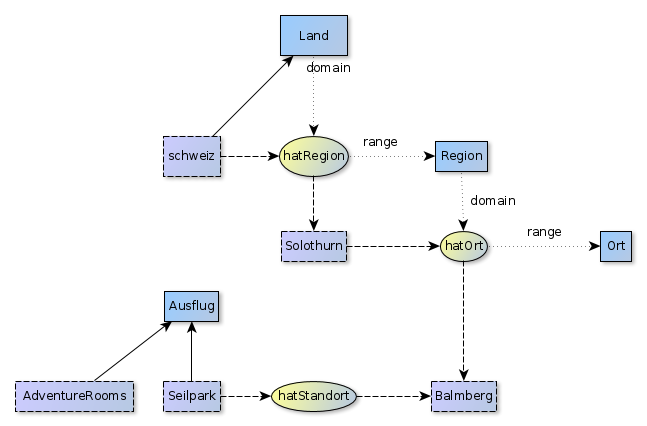
\includegraphics{bilder/beispiel_semantisches_netz.png}}}
\caption{Abbildung von Wissen mittels eines semantischen Netzes.\label{fig:semantischesNetz}\protect\footnotemark}
\end{figure}
\footnotetext{Eigene Darstellung mittels yEd}

Bei dieser Abbildung handelt es sich um eine Übersicht der \textit{Informationen}.

Wie kann ich aber schliessen, dass das Individuum \textit{Seilpark Balmberg} die \textit{Region} \textit{Solothurn} hat? Aus dem vorhandenen \textit{semantischen} Netz lässt sich dies nicht folgern. Somit fehlt die Möglichkeit einer Folgerung.

\vspace{0.1pt}
\noindent\rule[1ex]{\textwidth}{1pt}
